\documentclass[a4paper]{article}
\usepackage{ctex}
%\usepackage{svg}
\usepackage{amssymb,amsmath}
\usepackage{geometry}
\usepackage{graphicx}
\usepackage{color}
\usepackage{hyperref}
\begin{document}
以下的每个魔法题目前面都有标注难度,难度的含义是相对于同类的魔法题目,并不是绝对的难度。
题目中涉及到的几何图形均省略,因为这些图形都很简单,描述起来不会产生歧义。

有些题目之前已经说过,故此略去解答。

\section{初中魔法}
\begin{enumerate}
\item (easy)$\triangle ABC$是等腰三角形,而且它可以被分成两个等腰三角形。则$\triangle ABC$
顶角的所有可能值是多少?\\
\textbf{解}\quad $36^\circ,90^\circ,108^\circ,180^\circ/7$.
\item (easy)现在有足够多的正五边形地砖和正十边形地砖,它们的边长都相等。请问能否用它们覆盖整个平面(地砖之间
不能有重叠)?为什么?\\
\textbf{解}\quad 不能。不信你自己铺一下试试/w$\backslash$
\item (medium)在$\triangle ABC$中,$AD$是$\angle BAC$的平分线,求证:$\frac{AB}{AC}=\frac{BD}{DC}$。
(注:禁止使用相似三角形)。\\
\textbf{解}\quad 过点$D$作$DM\bot AB$,$DN\bot AC$。考虑$\triangle ABD$与$\triangle ACD$的比值。\\
\[
\frac{AB\cdot DM}{AC\cdot DN}=\frac{S_{\triangle ABD}}{S_{\triangle ACD}}=\frac{BD}{DC}
\]
$\because AD$为角平分线,$\therefore DM=DN$,上式左侧约去这两项即得结论。
\item (medium)设函数$y=ax^2+bx+c$的图像如下图。则$b^2-2ac$和$5a^2$的大小关系为?并证明你的结论。\\
\begin{figure}[!hbp]
\centering
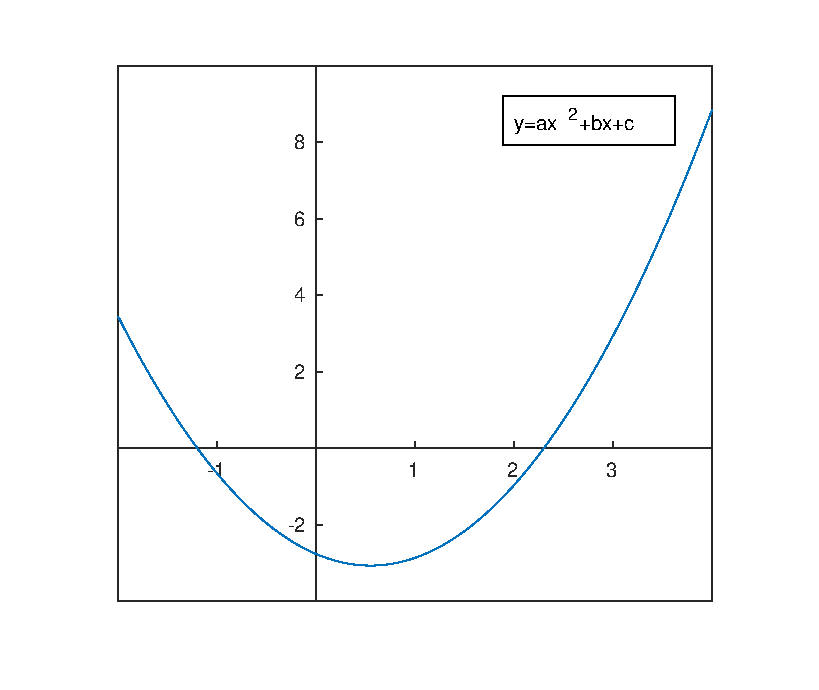
\includegraphics[width=0.5\textwidth]{quad.eps}
\end{figure}
\textbf{解}\quad 从图中可知方程$ax^2+bx+c=0$有两个解$x_1,x_2$.\\
由韦达定理,我们有
\[
\left\{\begin{array}{l}
x_1+x_2=-b/a\\
x_1x_2=c/a\\
\end{array}
\right.
\]
$\therefore x_1^2+x_2^2=(x_1+x_2)^2-2x_1x_2=\frac{b^2}{a^2}-\frac{c}{a}=\frac{b^2-2ac}{a^2}$\\
再由图中可得$x_1<-1,x_2>2$,得$\frac{b^2-2ac}{a^2} > 1^2+2^2=5$,因此
\[
b^2-2ac>5a^2
\]

\item (hard)设$\triangle ABC$是等腰三角形,$AB=AC,\angle A=80^\circ$。点$O$为$\triangle ABC$内部
一点,且$\angle OBC=10^\circ,\angle OCA=20^\circ$。求$\angle BAO$的度数。\\
\textbf{解}\quad 略。请询问叶子姐姐和九姐姐。
\end{enumerate}
\section{高中魔法}
\begin{enumerate}
\item (easy)设$a,b,c$是实数,则$a^3+b^3+c^3=3abc$的条件为?\\
\textbf{解}\quad 使用因式分解即可。
\[
\begin{split}
&a^3+b^3+c^3-3abc\\
=&(a+b)^3-3a^b-3ab^2+c^3-3abc\\
=&(a+b)^3+c^3-3ab(a+b+c)\\
=&(a+b+c)((a+b)^2-c(a+b)+c^2)-3ab(a+b+c)\\
=&(a+b+c)(a^2+b^2+c^2-ac-bc-ab)\\
=&(a+b+c)((a-b)^2+(b-c)^2+(c-a)^2)/2\\
\end{split}
\]
由以上分解式可知,上式为0的条件为$a=b=c$或$a+b+c=0$
\item (easy)设集合$M=\{1,2\}$,定义集合$A=\{x~|~\forall a \in x, a \in M \}$。则集合$A$和
$M$的关系为?\\
\textbf{解}\quad 由题目可知集合$A$是集合$M$所有子集构成的集合,因此$M$是$A$的一个元素。答案为$M\in A$
\item (medium)求值:$\cos\frac{2}{7}\pi+\cos\frac{4}{7}\pi+\cos\frac{6}{7}\pi$\\
\textbf{解}\quad 利用三角恒等变形,积化和差公式,裂项相消。
\[
\begin{split}
&\cos\frac{2}{7}\pi+\cos\frac{4}{7}\pi+\cos\frac{6}{7}\pi\\
=&\frac{\sin\frac{\pi}{7}(\cos\frac{2}{7}\pi+\cos\frac{4}{7}\pi+\cos\frac{6}{7}\pi)}{\sin\frac{\pi}{7}}\\
=&\frac{\sin\frac{\pi}{7}\cos\frac{2}{7}\pi+\sin\frac{\pi}{7}\cos\frac{4}{7}\pi+\sin\frac{\pi}{7}\cos\frac{6}{7}\pi}{\sin\frac{\pi}{7}}\\
=&\frac{\sin\frac{3\pi}{7}-\sin\frac{\pi}{7}+\sin\frac{5\pi}{7}-\sin\frac{3\pi}{7}+\sin\frac{7\pi}{7}-\sin\frac{5\pi}{7}}{2\sin\frac{\pi}{7}}\\
=&\frac{0-\sin\frac{\pi}{7}}{2\sin\frac{\pi}{7}}\\
=&-\frac{1}{2}\\
\end{split}
\]
\item (medium)设椭圆$E:\frac{x^2}{a^2}+\frac{y^2}{b^2}=1,a>b>0$,点$P(x_0,y_0)$在椭圆
上。过点$P$分别引出两条斜率为$k_1,k_2$的直线,满足$k_1+k_2=0$。两条直线分别交椭圆于点$A$和$B$。
求证:$AB$的斜率是定值。\\
\textbf{证明}\quad 利用椭圆的参数方程。\\
设$A=(a\cos \alpha,b\sin \alpha),~B=(a\cos \beta,b\sin\beta),~P=(a\cos \eta,b\sin\eta)$,其中
可以认为$x_0=a\cos\eta,y_0=b\sin\eta$\\
计算出两条线的斜率
\[
\left\{\begin{array}{l}
k_1=\frac{b}{a}\cdot \frac{\sin\alpha-\sin\eta}{\cos\alpha-\cos\eta}\\
k_2=\frac{b}{a}\cdot \frac{\sin\beta-\sin\eta}{\cos\beta-\cos\eta}\\
\end{array}
\right.
\]
代入$k_1+k_2=0$,我们有
\[
\frac{\sin\alpha-\sin\eta}{\cos\alpha-\cos\eta}+\frac{\sin\beta-\sin\eta}{\cos\beta-\cos\eta}=0
\]
对分子,分母使用和差化积公式,可得
\[
\frac{\cos(\frac{\alpha+\eta}{2})\sin(\frac{\alpha-\eta}{2})}{\sin(\frac{\alpha+\eta}{2})\sin(\frac{\alpha-\eta}{2})}+\frac{\cos(\frac{\beta+\eta}{2})\sin(\frac{\beta-\eta}{2})}{\sin(\frac{\beta+\eta}{2})\sin(\frac{\beta-\eta}{2})}=0
\]
以上可以等价写作
\[
\cot(\frac{\alpha+\eta}{2})=-\cot(\frac{\beta+\eta}{2})
\]
由三角函数诱导公式,可得
\[
\frac{\alpha+\eta}{2}+\frac{\beta+\eta}{2}=k\pi
\]
以上可以等价写作
\[
\frac{\alpha+\beta}{2}=k\pi-\eta
\]
同时,计算直线$AB$的斜率,可知
\[
k_{AB}=\frac{b}{a}\cdot \frac{\sin\alpha-\sin\beta}{\cos\alpha-\cos\beta}
\]
再次使用和差化积公式,我们有
\[
k_{AB}=\frac{b}{a}\cdot -\frac{\cos(\frac{\alpha+\beta}{2})\sin(\frac{\alpha-\beta}{2})}{\sin(\frac{\alpha+\beta}{2})\sin(\frac{\alpha-\beta}{2})}=-\frac{b}{a}\cdot \cot(\frac{\alpha+\beta}{2})
\]
代入$\frac{\alpha+\beta}{2}=k\pi-\eta$,并注意到$\cot\eta=\frac{bx_0}{ay_0}$,我们最终有
\[
k_{AB}=-\frac{b}{a}\cdot \cot(\frac{\alpha+\beta}{2})=-\frac{b}{a}\cdot \cot(k\pi-\eta)=\frac{b^2x_0}{a^2y_0}
\]
\item (hard)设数列$\{a_n\}$满足递推式\color{red}$a_{n+1}=a_n^2-2,a_0=a$\color{black}。求$a_n$的表达式。\\
\textbf{解}\quad 原题目符号打错了。解题方法是对$a$进行讨论。
\begin{itemize}
\item $|a|=2$,此时用归纳法证明$a_n=2,n > 0$
\item $|a|<2$,此时令$a=2\cos\eta$,使用归纳法证明$a_n=2\cos(2^{n}\eta)$
\item $|a|>2$,此时令$a=x_0+1/x_0$,使用归纳法证明$a_n=x_0^{2^n}+1/x_0^{2^n}$
\end{itemize}
细节从略。
\end{enumerate}
\section{大学魔法}
\begin{enumerate}
\item (easy)下列说法是否正确?如果正确请证明这个结论,如果不正确请举出反例。
	\begin{enumerate}
	\item 设数列$a_n\rightarrow 0$,$S_n=\sum_{i=1}^{n}a_i$,则$S_n$一定有极限。\\
	\textbf{错误}\quad 反例为$a_n=1/n$
	\item 设函数$f(x)$在$\mathbb{R}$上可导,并且有$\lim_{x\rightarrow +\infty}f(x)=0$,
	则有$\lim_{x\rightarrow +\infty}f'(x)=0$。\\
	\textbf{错误}\quad 导数$f'(x)$在无穷处可能没有极限。反例为$f(x)=\frac{\sin x^2}{x}$。
	\item 可导函数$f(x)$在$\mathbb{R}$上为凸函数当且仅当$f'(x)$是单调递增的。\\
	\textbf{正确}\quad 这是凸函数的一个判定定理。\\
	\emph{必要性}~~由凸函数性质,对于任意的$x,y$
	\[
	\left\{\begin{array}{l}
	f(y)-f(x)\geq f'(x)(y-x)\\
	f(x)-f(y)\geq f'(y)(x-y)\\
	\end{array}
	\right.
	\]
	两式相加,可得
	\[
	0\leq (f'(x)-f'(y))(x-y)
	\]
	这说明$f'(x)$单调递增。\\
	\emph{充分性}~~由凸函数判定定理,对于任意$x_1<x_2<x_3$,如果以下有关斜率的不等式成立
	\[
	\frac{f(x_1)-f(x_2)}{x_1-x_2}\leq \frac{f(x_2)-f(x_3)}{x_2-x_3}
	\]
	那么$f(x)$为凸函数。\\
	而根据Lagrange中值定理和$f'(x)$的单调性,这是显然的。
	\item 设$A\in \mathbb{R}^{n\times n}$,则$A$可以分解为一个对称矩阵和一个反对称矩阵的和。并且这个分解是
	唯一的。\\
	\textbf{正确}\quad 这是矩阵的一种直和分解。\\
	\emph{存在性}~~考虑恒等式$A=\frac{A+A^T}{2}+\frac{A-A^T}{2}$,令$B=\frac{A+A^T}{2},C=\frac{A-A^T}{2}$,
	则显然$B$对称,$C$反对称。\\
	\emph{唯一性}~~设$A=B_1+C_1=B_2+C_2$,其中$B_1,B_2$对称,$C_1,C_2$反对称。我们有
	\[
	B_1-B_2=C_2-C_1
	\]
	注意到等式左边是对称矩阵,等式右边是反对称矩阵。一个矩阵既是对称又是反对称,它只能是零矩阵。因此$B_1=B_2,C_1=C_2$。
	\end{enumerate}
\item (easy)已知矩阵$A,B$均为半正定矩阵,求证$\mathrm{tr}(AB)\geqslant0$。\\
\textbf{证明}\quad 略。使用特征值分解与$\mathrm{tr}(\cdot)$的可交换性。
\item (medium)设连续函数$f(x)$满足$f(x+y)=f(x)+f(y),\forall x,y \in \mathbb{R}$,求证:
$f(x)=kx$,其中$k\in \mathbb{R}$为一常数。\\
\textbf{证明}\quad 设$k=f(1)$下面分为几个部分证明。仅提供思路,细节请自己完成。
\begin{enumerate}
\item $f(x)=kx$对所有$x\in\mathbb{N}$成立,使用归纳法,这是显然的。此外你可能需要推导$f(x)$的奇偶性。
\item $f(x)=kx$对所有$x\in\mathbb{Q}$成立,需要使用(a)中的结论。
\item $f(x)=kx$对所有$x\in\mathbb{R}$成立,需要使用(b)中的结论,以及使用有理数逼近实数。最重要的,需要函数的连续性。
\end{enumerate}
\item (medium)设矩阵$A$的每个元素为$a_{ij}$,对于任意的$i$,满足$|a_{ii}|>\sum_{j\neq i}{|a_{ji}|}$。
求证:$A$是非奇异矩阵。\\
\textbf{证明}\quad 使用Gershgorin圆盘定理即可。\\
设$\lambda$为矩阵任意特征值,则由Gershgorin定理,有$|\lambda - a_{ii}|<\sum_{j\neq i}{|a_{ji}|}$。这里$i$是某一个下标。
但是由条件$|a_{ii}|>\sum_{j\neq i}{|a_{ji}|}$可得此时$\lambda$不可能为0。所以$A$没有零特征值,故而非奇异。
\item (medium)设$X$为概率空间$(\Omega,\mathcal{F},P)$上的随机变量,$f(x)$是凸函数。求证:
$f(\mathbb{E}X)\leqslant \mathbb{E}f(X)$,其中$\mathbb{E}(\cdot)$表示对随机变量求期望。\\
\textbf{证明}\quad \url{https://en.wikipedia.org/wiki/Jensen's_inequality}
\item (medium)设二元函数$f(x,y)$是凸函数,$C$是凸集。令$g(x)=\inf_{y\in C}f(x,y)$,求证:
$g(x)$为凸函数。\\
\textbf{证明}\quad 利用凸函数定义即可。\\
对于任意$x_1,x_2$,任取$\varepsilon>0$,存在$y_1,y_2\in C$,使得$f(x_i,y_i)\leqslant g(x_i)+\varepsilon,~~i=1,2$。\\
因此考虑$\lambda \in (0, 1)$,验证凸函数定义:
\[
\begin{split}
&g(\lambda x_1+(1-\lambda)x_2)=\inf_{y\in C}f(\lambda x_1+(1-\lambda) x_2, y)\\
\leqslant &f(\lambda x_1+(1-\lambda)x_2,\lambda y_1+(1-\lambda)y_2)\\
\leqslant &\lambda f(x_1,y_1)+(1-\lambda)f(x_2,y_2)\\
\leqslant &\lambda (g(x_1)+\varepsilon)+(1-\lambda)(g(x_2)+\varepsilon)\\
=&\lambda g(x_1)+(1-\lambda) g(x_2)+\varepsilon\\
\end{split}
\]
由$\epsilon$的任意性,我们就得到了$g(x)$的凸性。
\end{enumerate}
\end{document}